Multicast Domain Name System (mDNS, \href{https://tools.ietf.org/html/rfc6763}{RFC 6763}) es el protocolo usado para encontrar los dispositivos a los que conectarnos.

mDNS transforma nombres de dominio en direcciones IP dentro de su registro de direcciones IPv4 o IPv6 usando el puerto 5353. Está pensado para redes locales sin tener que incluir un servidor DNS.
Tiene las mismas interfaces de programación, formatos y restricciones semánticas que DNS, pero permite designar una porción del espacio de nombres de DNS a nuestro gusto, sin tener que pagar anualmente.

Usa UDP en multicast y sus ventajas son:
\begin{itemize}
	\item Necesita poca configuración para activarse
	\item Funciona cuando no hay infraestructura
	\item Soporta fallos en la infraestructura
\end{itemize}

En el primer caso envía a todos los dispositivos una solicitud para identificarse.

\begin{figure}[H]
	\centering
	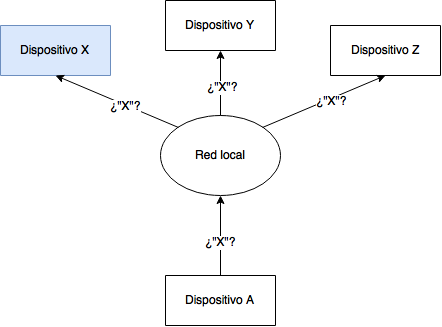
\includegraphics[width=0.6\textwidth]{./Imagenes/mdns1.png}
	\label{fig:mdns1}
	\caption{Primer paso del protocolo mDNS}
\end{figure}


Ejemplo de petición:

00 00 \textbf{00 00}(1) 00 01 00 00 \hspace{0.1cm} 00 00 00 00  \textbf{07 61 70 70}

\textbf{6c 65 74 76}(2) \textbf{05 6c 6f 63} \hspace{0.1cm} \textbf{61 6c}(3) 00 00 01 00 01
			
\begin{itemize}
	\item Flag de petición(1)
	\item Nombre de dominio del servidor (appletv(2).local(3))
\end{itemize}


Como respuesta se devuelve la dirección IP con una variable TTL (Time To Live) para saber cuánto tiempo durará vigente la IP enviada.

Si un dispositivo quiere rechazar la petición manda una IP con TTL cero.

\begin{figure}[H]
	\centering
	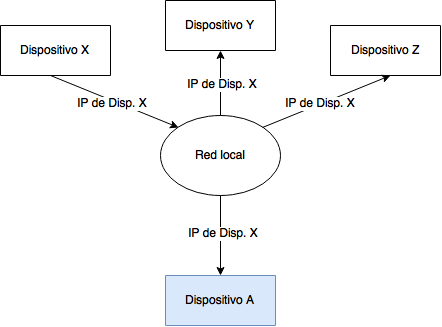
\includegraphics[width=0.6\textwidth]{./Imagenes/mdns2.png}
	\label{fig:mdns2}
	\caption{Segundo paso del protocolo mDNS}
\end{figure}


	Ejemplo respuesta:

	00 00 \textbf{84 00}(1) 00 00 00 01 \hspace{0.1cm} 00 00 00 02 07 61 70 70
	
	6c 65 74 76 05 6c 6f 63 \hspace{0.1cm} 61 6c 00 00 01 80 01 00
	
	00 78 00 00 04 \textbf{99 6d 07} \hspace{0.1cm} \textbf{5a}(2) c0 0c 00 1c 80 01 00
	
	00 78 00 00 10 \textbf{fe 80 00} \hspace{0.1cm} \textbf{00 00 00 00 00 02 23 32}
	
	\textbf{ff fe b1 21 52}(3) c0 0c 00 \hspace{0.1cm} 2f 80 01 00 00 78 00 00
	
	08 c0 0c 00 04 40 00 00 \hspace{0.1cm} 08

	
\begin{itemize}
	\item (1) Flag de respuesta
	\item (2) Bytes de dirección IPv4
	\item (3) Bytes de dirección IPv6
\end{itemize}
